\section{Organisatorisches}
Prof. Bauer, Raum Z442 (440, 431)

Modul besteht aus den Units Gerätekonstruktion \emph{und} Werkstofftechnik, d.h. es gibt nur eine Prüfung.

2 GK Praktika im Laufe des Semesters mit je 2 SWS, beginnend KW44.

GK-Übung findet 14-tägig statt.

Skript gibt's im Downloadbereich. Siehe Sidebar rechts auf Prof.-Seite. \\Nutzername: grstudium

Literaturempfehlung: Gerätekonstruktion in der Feinwerktechnik und Elektronik. Siehe Skript für Details.

\section{Einführung in die Gerätekonstruktion}

3 Axiome der Konstruktionswissenschaft

\begin{enumerate}
	\item Ganzheitsaxiom:
		Gesamtes System betrachten, nicht nur Einzelteil
	\item Zeitwertaxiom:
		Jede Entwicklung wird langfristig durch Bessere ersetzt
	\item Fehleraxiom:
		Es gibt immer Abweichungen zu beachten
\end{enumerate}

$\Rightarrow$ Ein Produkt hat Bestand am Markt, wenn es Kunden einen sinnvollen und anwendungsgerechten Nutzen für die geplante Nutzungsdauer zu einem bezahlbaren Preis bietet. (realisierter Gebrauchswert)

\section{Systembetrachtung elektronischer und elektromechanischer Geräte}
\subsection{Funktionsstrukturen}

\underbar{a) Allgemeines Modell eines technischen Systems}

\begin{center}
	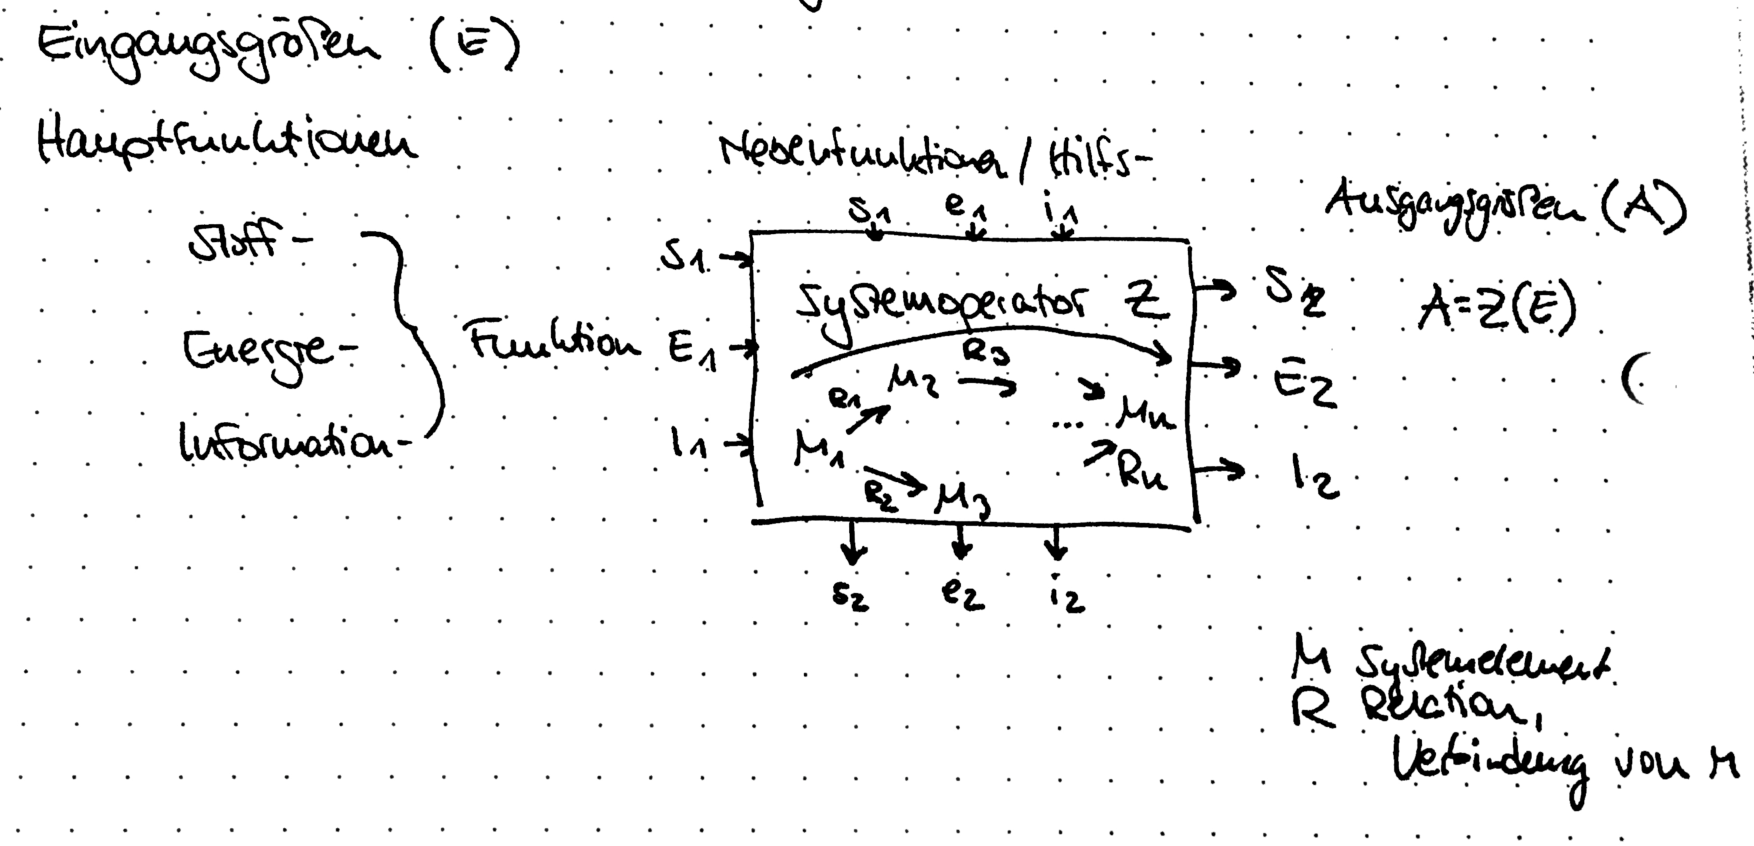
\includegraphics[width=.8\textwidth]{img/1_1}
\end{center}
